\documentclass{standalone}
\usepackage{tikz}
\usepackage{pgfplots}
\pgfplotsset{width=15cm,compat=1.18}
\begin{document}

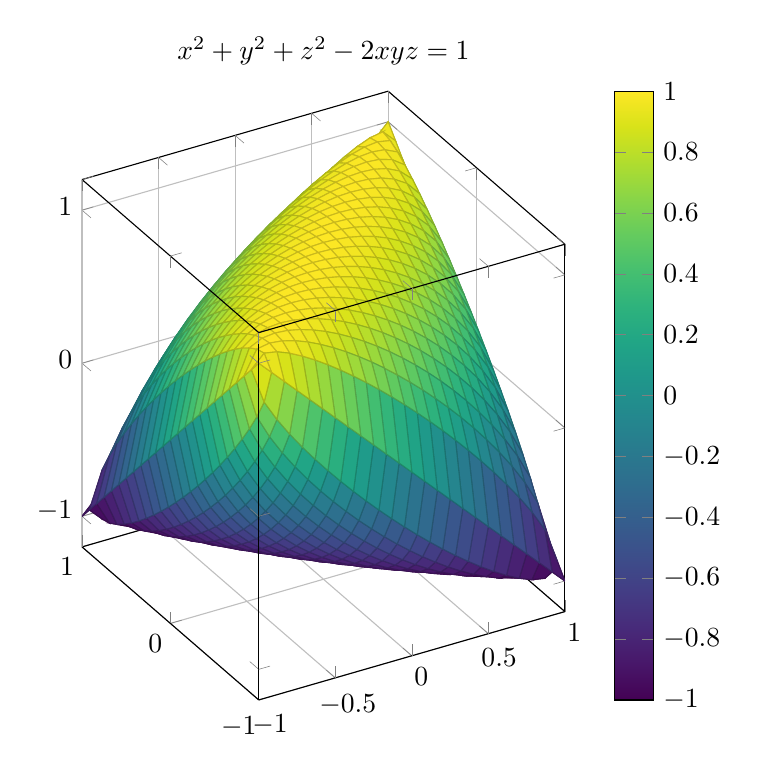
\begin{tikzpicture}
\begin{axis}
[ 
  view/h=-30,
  colormap/viridis,
  colorbar,
  3d box,
  samples=25,
  axis equal image,
  z buffer=sort,
  grid=major,
  title={$x^2+y^2+z^2-2xyz=1$},
  % opacity=0.7,
  % shader=interp,
]
\addplot3 [surf,domain=-1:1] (
 {x},
 {y},
 {x*y - sqrt((x^2-1)*(y^2-1))}
);
\addplot3 [surf,domain=-1:1] (
 {x},
 {y},
 {x*y + sqrt((x^2-1)*(y^2-1))}
);
\end{axis}
\end{tikzpicture}

\end{document}
